% Kinematic fitting at ANKE
\begin{itemize}
\item Reaction $pp \to pp$ at ANKE;
\item Polar CMS coordinates;
\item Undetected proton;
\item A constraint $\left|\boldsymbol{P}^{(4)}_\mathrm{beam}+\boldsymbol{P}^{(4)}_\mathrm{targ}-\boldsymbol{P}^{(4)}_p\right|^2 = m_p^2$.
\end{itemize}

\centering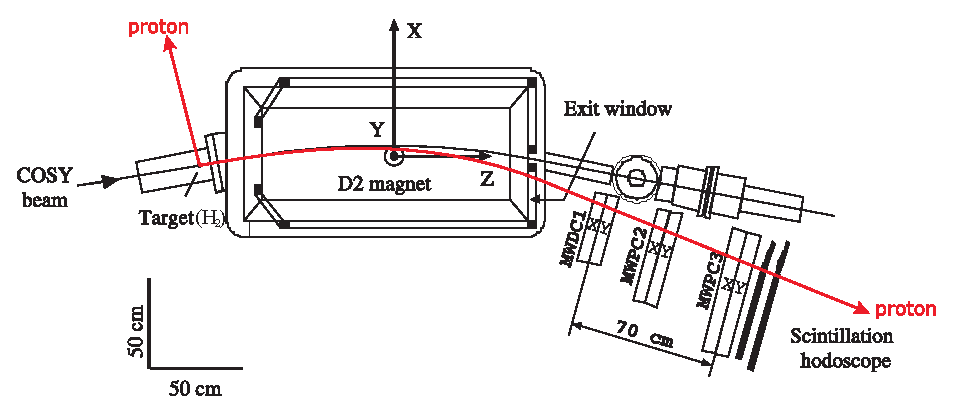
\includegraphics[width=0.8\textwidth]{pics/setup_.eps}

% \large
% \phantom{0}
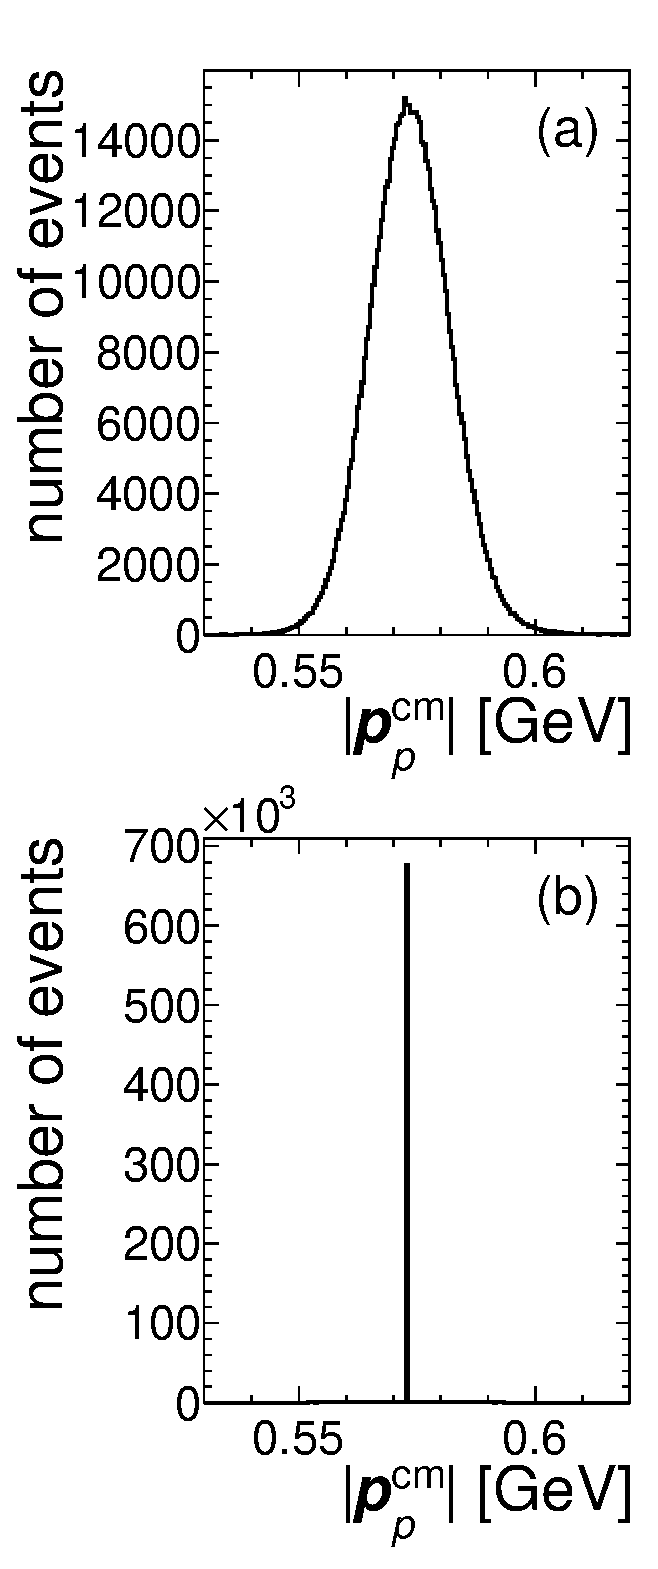
\includegraphics[height=0.7\textheight]{pics/drawMom.eps}
\hfill
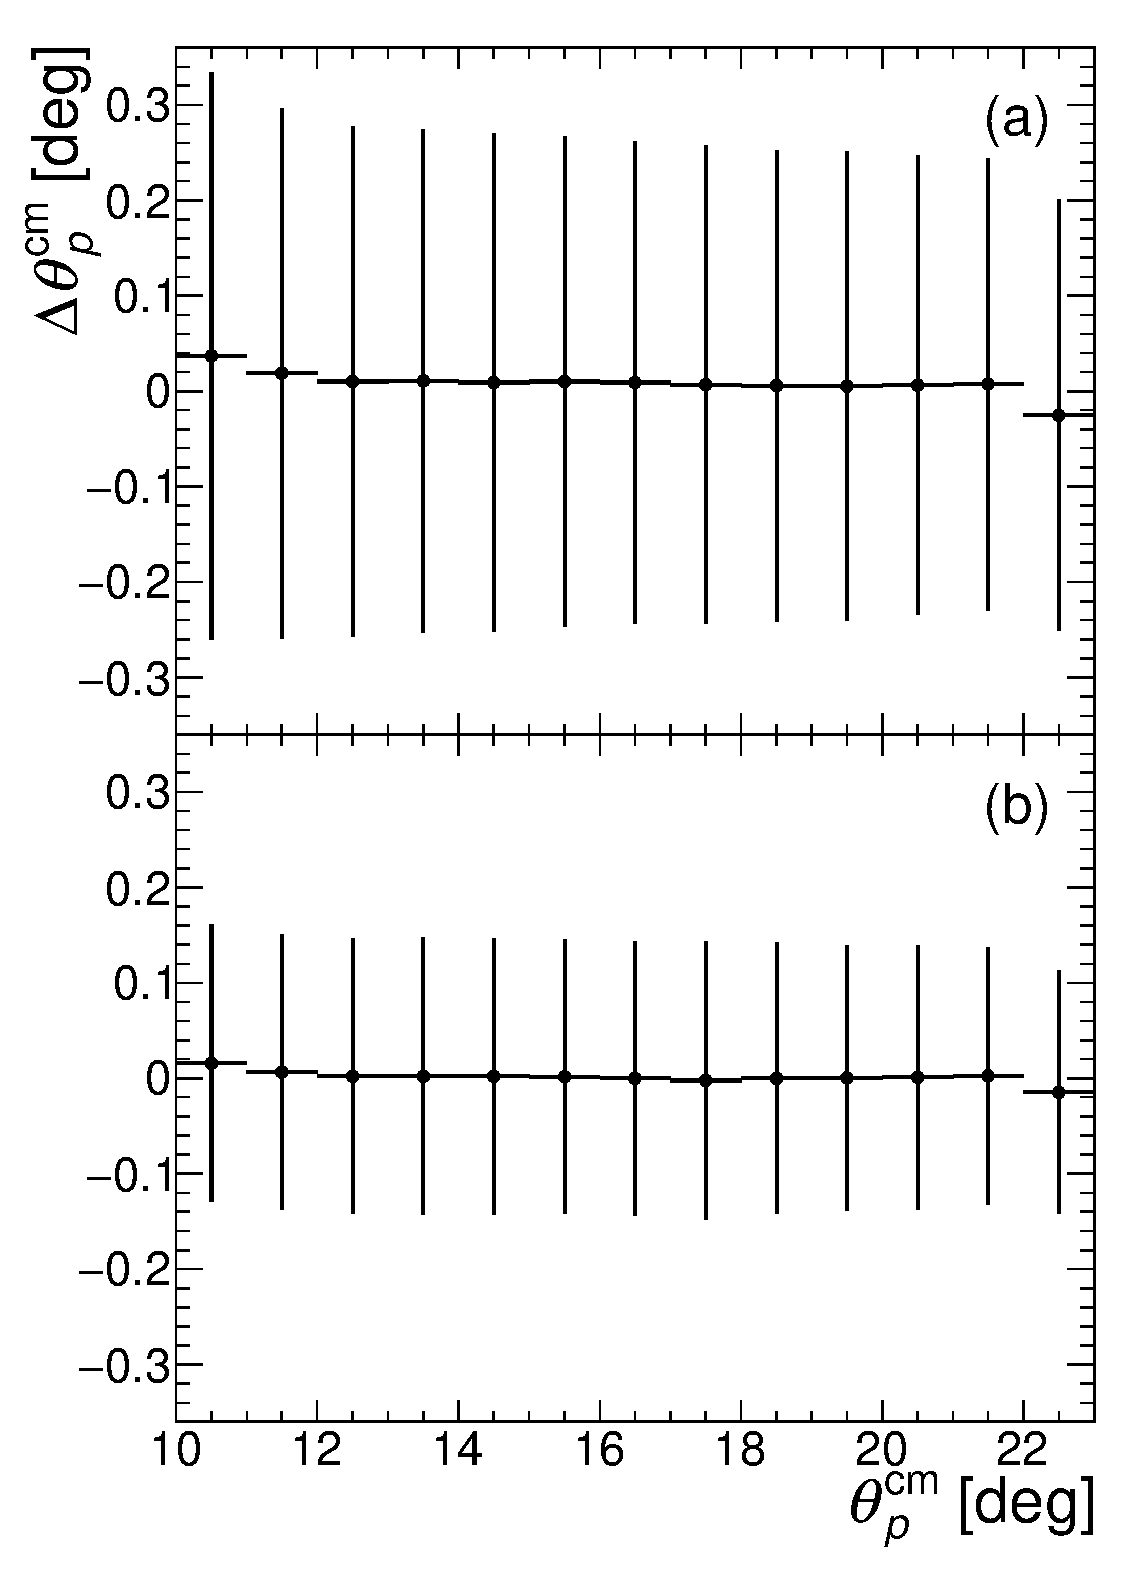
\includegraphics[height=0.7\textheight]{pics/drawTh.eps}
\hfill
% \hspace{1em}
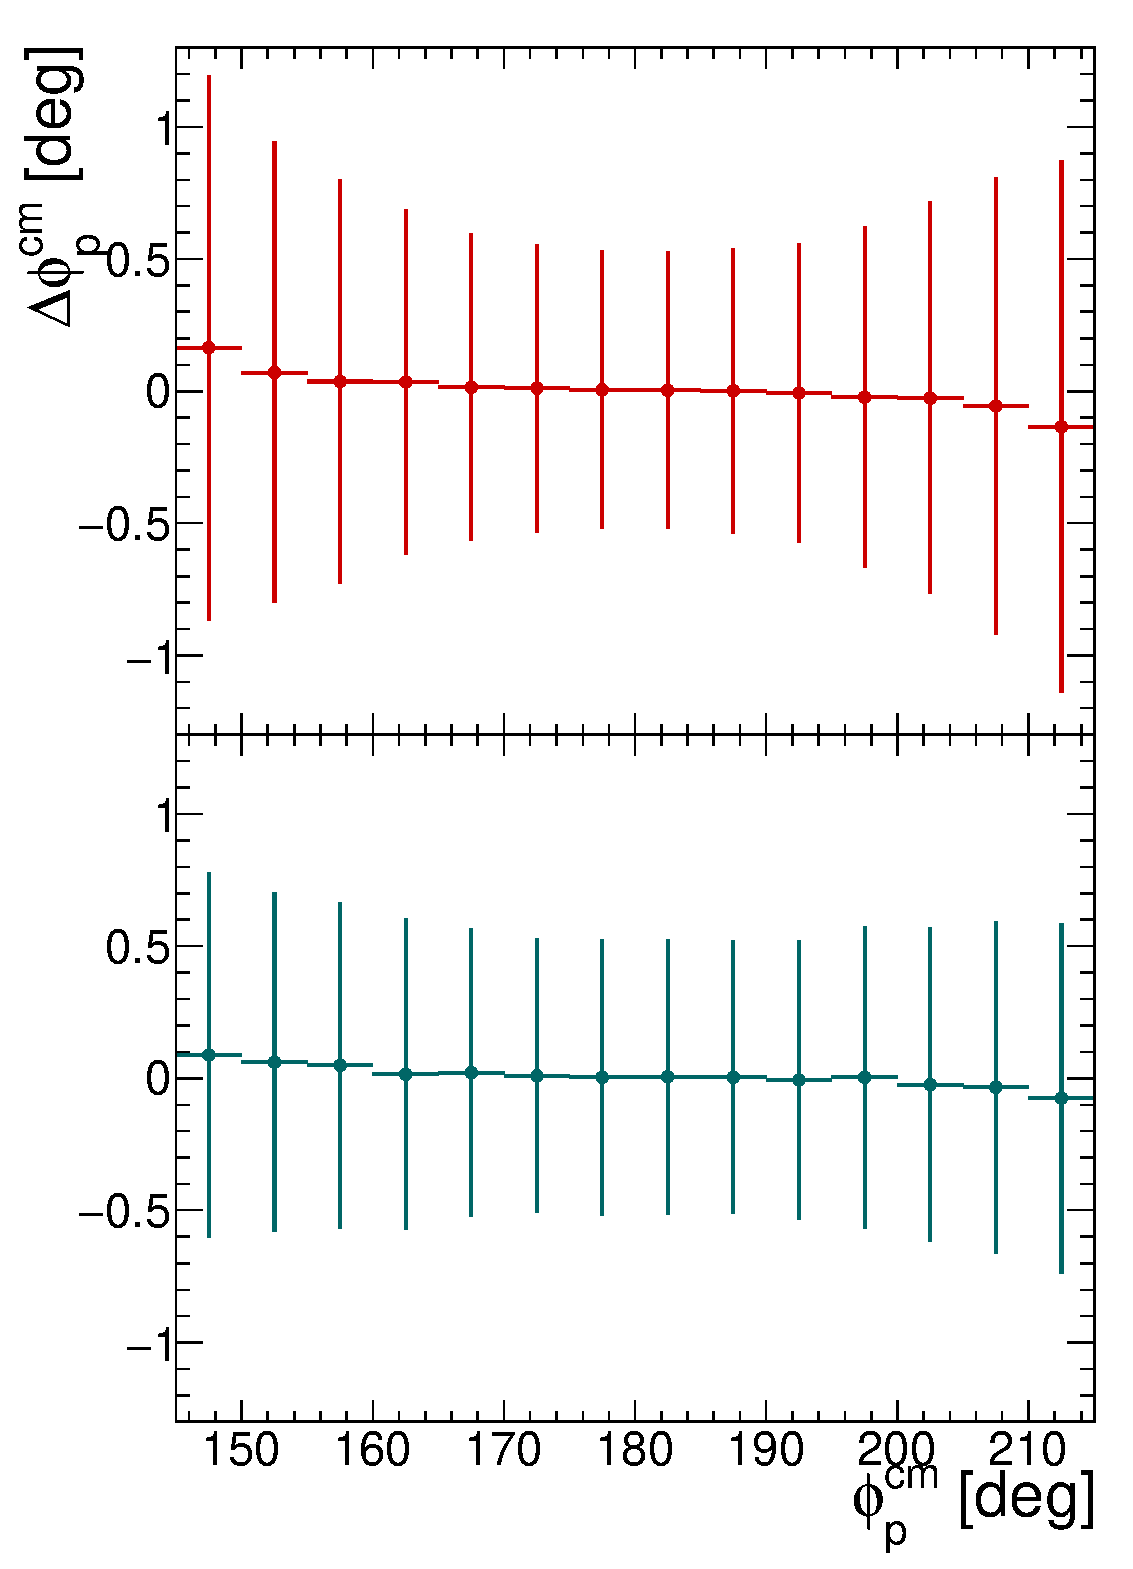
\includegraphics[height=0.7\textheight]{pics/drawPhi.eps}
% \hfill
% \phantom{0}

Errors of reconstructed proton momentum in polar coordinates $(|P_p^\mathrm{cm}|, \theta_p^\mathrm{cm}, \phi_p^\mathrm{cm})$ for the $pp \to pp$ reaction at ANKE, simulated for $T_\mathrm{beam} = 700$~MeV with and without kinematic fitting.
